\documentclass[11pt]{amsart}
\usepackage{amsmath,amssymb,amsthm,mathtools}
\usepackage[margin=1in]{geometry}
\usepackage{hyperref}
\usepackage{array}
\usepackage{booktabs}
\usepackage{longtable}
\usepackage{xcolor}
\usepackage{enumitem}
\usepackage{tikz}
\usetikzlibrary{arrows.meta,positioning,shapes.geometric,fit,backgrounds}

%% Theorem environments
\newtheorem{theorem}{Theorem}[section]
\newtheorem{proposition}[theorem]{Proposition}
\newtheorem{lemma}[theorem]{Lemma}
\newtheorem{corollary}[theorem]{Corollary}
\newtheorem{conjecture}[theorem]{Conjecture}
\theoremstyle{definition}
\newtheorem{definition}[theorem]{Definition}
\newtheorem{example}[theorem]{Example}
\theoremstyle{remark}
\newtheorem{remark}[theorem]{Remark}
\newtheorem{notation}[theorem]{Notation}


%% Math macros
\newcommand{\RH}{\mathrm{RH}}
\renewcommand{\Re}{\operatorname{Re}}
\renewcommand{\Im}{\operatorname{Im}}
\newcommand{\half}{\tfrac{1}{2}}
\newcommand{\om}{\omega}
\newcommand{\kap}{\kappa}
\newcommand{\gam}{\gamma}
\newcommand{\Lam}{\Lambda}
\newcommand{\eps}{\varepsilon}
\newcommand{\Spec}{\operatorname{Spec}}
\newcommand{\Fq}{\mathbb{F}_q}
\newcommand{\Tr}{\operatorname{Tr}}
\newcommand{\Ad}{\mathbb{A}}
\newcommand{\Q}{\mathbb{Q}}
\newcommand{\R}{\mathbb{R}}
\newcommand{\Z}{\mathbb{Z}}
\newcommand{\C}{\mathbb{C}}
\newcommand{\Hil}{\mathcal{H}}
\newcommand{\Dm}{\mathcal{D}}
\newcommand{\Xibar}{\Xi}
\newcommand{\Th}{\Theta}
\newcommand{\Sk}{S_\kap}
\newcommand{\Ek}{E_\kap}
\newcommand{\indm}{\operatorname{ind}_-}
\DeclareMathOperator{\ind}{ind}

\title[The Colligation Route to RH]{The Colligation Route to the Riemann Hypothesis:\\
de Branges Realization, a Curvature Theorem, and the\\
Pole-Pinned Spectral Radius at the Wall}

\author{David Alejandro Trejo Pizzo}
\thanks{Independent Researcher. \texttt{dtrejopizzo@gmail.com}}

\begin{document}
\maketitle

\begin{abstract}
We develop and rigorously assemble a single route to the Riemann Hypothesis (RH) built on the
de~Branges / Lax--Phillips colligation attached to the completed zeta function $\xi$, and we
localize the remaining obstruction with full precision. Four results are unconditional and new
or newly-sharpened. \textbf{(A)} The finite-window boundedness $L1$ of the oscillatory part of
the Weil form \emph{implies} RH ($L1\Rightarrow\RH$, the Laplace--pole theorem), whose only non-formal
input --- a Paley--Wiener nonvanishing lemma --- is proved unconditionally (the converse
$\RH\Rightarrow L1$ is conditional on a regularized zero-sum estimate). \textbf{(B)} The correct index of the route is the Kre\u\i n--Langer
negative-square count $\indm(K_{\Sk})=\#\{\text{off-line zeros}\}$, so $\RH\Leftrightarrow
\indm=0$. \textbf{(C)} After Doob conjugation the prime part of the Weil generator is a
Beurling--Deny Dirichlet form whose iterated carr\'e-du-champ satisfies
$\Gamma_2\ge 0$ \emph{unconditionally} (a Bakry--\'Emery $CD(0,\infty)$ curvature bound), by a
Schur-product mechanism rooted in $\Lam\ge 0$; the Davenport--Heilbronn falsifier fails this bound.
\textbf{(D)} The wall $\eps_0(\lambda)\ge 0$ (Weil positivity) is realized as the absence of a
\emph{Schr\"odinger bound state}, equivalently $\|K_\lambda(0)\|\le 1$ for an explicit
Birman--Schwinger operator, in which the pole of $\zeta$ at $s=1$ acts as a repulsive barrier
pinning the spectral radius from below at $1$, and the Perron--Frobenius ground state $u_0$ is the
threshold resonance.

The synthesis is a single sharp statement: \emph{every geometric and functional-analytic structure
on the route is Doob-invariant and therefore proves the unconditional ``shape'' (the $(k+1)^2$
ladder, the curvature, the colligation), while RH is the ``sign'' $\eps_0\ge0$ --- the
\emph{upper} pinning of the Birman--Schwinger spectral radius at $1$.} In the function-field model
this upper pinning is the Weil pairing (Frobenius is a $\sqrt q$-isometry); over $\Spec\Z$ it is
missing. We state the missing object precisely (an arithmetic intersection pairing on the square of
the arithmetic site, with a Hodge-index sign), give a candidate construction, and argue that
crossing the wall requires \emph{creating} this piece of arithmetic geometry. Nothing here proves
RH; the boundary is mapped exactly.
\end{abstract}

\tableofcontents
\newpage

%% =====================================================================
\section*{Preface}
%% =====================================================================
This is not a proof of the Riemann Hypothesis. It is a precise, honest account of a single
route --- the de~Branges/colligation route in the form proposed by Connes --- carried as far as it
rigorously goes, together with the exact localization of what remains. The programme operates under
one non-negotiable rule: \emph{a false positive is worse than a failure}. Every statement is either
proved (and labelled Theorem/Lemma/Proposition) or explicitly flagged as Conjecture or Open target.
Several places record corrections of the authors' own earlier proposals; these are structural data,
not embarrassments. The companion letter to A.~Connes summarizes the strategic picture and the map.

%% =====================================================================
\section{Foundations: the window, the Weil form, and the wall}
%% =====================================================================

\subsection{The completed zeta function and the spectral window}
Let $\xi(s)=\half s(s-1)\pi^{-s/2}\Gamma(s/2)\zeta(s)$ be the completed Riemann zeta function:
entire of order $1$, $\xi(s)=\xi(1-s)$, real on $\R$ and on the critical line $\Re s=\half$. Write
\[
   \Xibar(z):=\xi(\half+iz),\qquad \phi(z):=\frac{\Xibar'(z)}{\Xibar(z)},\qquad
   m(z):=-\phi(z).
\]
RH is the statement that all zeros of $\Xibar$ are real.

Fix $\lambda>1$ and set $L=2\log\lambda$. On the window $[0,L]$ with the Fourier basis
$e_n(y)=e^{2\pi iny/L}$ ($n=-N,\dots,N$), the Riemann--Weil explicit formula realizes the Weil
quadratic form as a symmetric matrix $A=A_\lambda$, split into archimedean/pole and prime parts,
\[
   A_\lambda=L_{\mathrm{arch}}-L_{\mathrm{prime}},\qquad
   A_\lambda[m,n]=A^{\mathrm{sm}}_\lambda[m,n]+A^{\mathrm{osc}}_\lambda[m,n],
\]
the smooth part governed by the prime number theorem (PNT) and the oscillatory part
$A^{\mathrm{osc}}_\lambda=-\sum_\rho c_{m,n}(\rho)\,\lambda^{2\rho-1}(1+o(1))$ the sum over
nontrivial zeros.

\subsection{Doob conjugation and the wall}
By Perron--Frobenius (the unconditional Theorem~2.2 of the programme), $A_\lambda$ has a simple
lowest eigenvalue $\eps_0=\eps_0(\lambda)$ with strictly positive eigenvector $u_0>0$. Doob
conjugation by $u_0$ produces the generator
\[
   G_\lambda:=u_0^{-1}(A_\lambda-\eps_0)u_0\ \succeq 0,
\]
a positive form whose internal structure (the $(k+1)^2$ Dirichlet ladder of Lemma~2.3.F) is
\emph{shape} data, while the additive constant $\eps_0$ is \emph{sign} data.

\medskip\noindent\textbf{Wall $W$: the sign $\eps_0\ge0$.}
The single surviving obstruction of the route is Weil positivity in window form:
\[
   \boxed{\ \eps_0(\lambda)\ge 0\ \text{ for all }\lambda\ \Longleftrightarrow\ \RH.\ }
\]
Equivalently $L_{\mathrm{prime}}\preceq L_{\mathrm{arch}}$, equivalently
$\mu_{\max}(L_{\mathrm{prime}},L_{\mathrm{arch}})\le1$. Numerically (companion computations,
not reproduced here) the value is marginal: $\mu_{\max}=1$ for $\zeta$.
\medskip

%% =====================================================================
\section{The de Branges / Lax--Phillips colligation}
%% =====================================================================

\subsection{Model space and the safe region}
For $\kap>0$ set $\Ek(z)=\Xibar'(z)-i\kap\Xibar(z)$, $\Ek^\#(z)=\overline{\Ek(\bar z)}
=\Xibar'(z)+i\kap\Xibar(z)$, and
\[
   \Sk(z)=\frac{\Ek^\#(z)}{\Ek(z)}=\frac{\phi(z)+i\kap}{\phi(z)-i\kap},\qquad
   K_S(z,w)=\frac{1-S(z)\overline{S(w)}}{2\pi i(\bar w-z)} .
\]
For the shifted family, $\Th_\om(z)=\xi(\half+\om+iz)/\xi(\half+\om-iz)$ ($\om>0$).

\begin{proposition}[de Branges--Rovnyak; safe region]\label{prop:model}
If $S$ is holomorphic with $|S|\le1$ on $\C_+$ (\emph{Schur}), then $K_S\succeq0$ and the
reproducing-kernel space $\mathcal H(S)$ is a Hilbert space; when $S$ is inner,
$\mathcal H(S)=H^2\ominus SH^2$ is a closed subspace of the Hardy space and carries a conservative
unitary colligation with transfer function $S$. Moreover $\Th_\om$ is inner on $\C_+$ for every
$\om>\tfrac12$.
\end{proposition}
\begin{proof}
The first statement is classical (Sz.-Nagy--Foia\c s, de~Branges--Rovnyak). For the second:
$|\Th_\om|=1$ on $\R$ since numerator and denominator are conjugates there; a pole of $\Th_\om$ is a
zero of $\xi(\half+\om-iz)$, located at $\Im z=\beta-\half-\om$ for a zero $\rho=\beta+i\gam$ with
$0<\beta<1$, hence in the lower half-plane when $\om>\half$. Thus $\Th_\om$ is bounded by $1$ and
holomorphic on $\C_+$.
\end{proof}

\subsection{The adelic realization and the angle reduction}
Let $\Hil=L^2(\Ad_\Q^\times/\Q^\times,d^\times x)$ with the scaling action $(U_tf)(x)=f(e^tx)$.
Define the Lax--Phillips incoming/outgoing subspaces
\[
   \Dm_-=\{f:f(x)=0\ \text{for } |x|>1\},\qquad \Dm_+=\mathcal F\,\Dm_-,
\]
$\mathcal F$ the adelic (Tate) Fourier transform. The scattering operator has characteristic
function $\Th_0$ (the ratio of completed zeta across the functional equation; Connes' spectral
realization / trace formula), and the interaction space is $K=\Hil\ominus(\Dm_-\oplus\Dm_+)$.

\begin{proposition}[angle criterion --- an equivalence, not an independent route]\label{thm:angle}
If $\Dm_-\oplus\Dm_+$ is a closed direct sum, then $K$ is a closed subspace of the Hilbert space
$\Hil$, the model identification $K\cong\mathcal H(\Th_0)$ is isometric, $K_{\Th_0}\succeq0$, and RH
holds. Consequently
\[
   \RH\ \Longleftrightarrow\ \angle(\Dm_-,\Dm_+)>0\ \Longleftrightarrow\
   \text{the overlap form on }\Dm_-\cap\overline{\Dm_+}\ \text{is}\ \succeq0 .
\]
\emph{This is a reformulation, not a proof route: the closedness / positive-angle hypothesis is itself
RH-strength} (it is equivalent to $K_{\Th_0}\succeq0$), so it must be supplied by an independent
construction. The Davenport--Heilbronn falsifier illustrates where such a construction must use
arithmetic: $\Dm_+=\mathcal F\Dm_-$ uses the adelic Fourier transform $\mathcal F=\bigotimes'_v
\mathcal F_v$, the \emph{Euler product over places}; a function with a functional equation but no Euler
product has no such $\Dm_+$.
\end{proposition}

\begin{remark}
The naive scalar Euler product diverges at the critical line, so $\Th_0$ on $\C_+$ is obtained by
analytic continuation, not literal product convergence; the Euler product enters only as the
restricted-tensor structure of $\mathcal F$. This is the corrected reading (Connes).
\end{remark}

%% =====================================================================
\section{$L1\Leftrightarrow\RH$: the Laplace--pole theorem}
%% =====================================================================
Let $B(t)=A^{\mathrm{osc}}_{e^t}$ and $\mathcal L B(w)=\int_0^\infty e^{-wt}B(t)\,dt$, with residue
$R_\rho=\operatorname{Res}_{w=2\rho-1}\mathcal LB$. Write \textbf{$L1$}: $\sup_\lambda\max_{m,n}
|A^{\mathrm{osc}}_\lambda[m,n]|<\infty$.

\begin{lemma}[Paley--Wiener nonvanishing; unconditional]\label{lem:pw}
For every nontrivial zero $\rho$ and all $m,n$, $R_\rho[m,n]\ne0$.
\end{lemma}
\begin{proof}
$R_\rho[m,n]=w(\rho)\,\hat e_m(\rho)\hat e_n(\rho)$ with $w(\rho)\ne0$ and the window transform
\[
   \hat e_n(\rho)=\int_0^L e^{2\pi iny/L}e^{\rho y}\,dy=\frac{e^{\rho L}-1}{\rho+2\pi in/L}.
\]
This vanishes iff $e^{\rho L}=1$, i.e.\ iff $\rho=2\pi ik/L$ is purely imaginary. A nontrivial zero
has $\Re\rho\in(0,1)$, hence is never purely imaginary, so $\hat e_n(\rho)\ne0$ for all $n$.
\end{proof}

\begin{theorem}[$L1\Rightarrow\RH$; the Laplace--pole theorem]\label{thm:L1}
If $L1$ holds, then RH holds.
\end{theorem}
\begin{proof}
If $L1$ holds, each entry $B[m,n](t)$ is bounded, so $\mathcal LB[m,n]$ is holomorphic in
$\Re w>0$; hence $R_\rho[m,n]=0$ for every zero with $\Re\rho>\half$. By Lemma~\ref{lem:pw} this
forces the absence of such zeros, and the functional equation removes $\Re\rho<\half$; thus RH.
\end{proof}

\begin{remark}[the converse, conditional --- Connes' audit]\label{rem:converse}
The reverse implication $\RH\Rightarrow L1$ is \emph{not} automatic from the boundedness of each
factor $\lambda^{2i\gam}$: the zero-sum is infinite and only conditionally (regularly) convergent, so
$L1$ requires a precise summation prescription and a uniform-in-$\lambda$ estimate of the regularized
zero-sum. We therefore state only $L1\Rightarrow\RH$ as proved, and regard the equivalence
$L1\Leftrightarrow\RH$ as established \emph{modulo} that regularized zero-sum estimate, which is left
open. The forward (and load-bearing) direction is unconditional.
\end{remark}

\begin{remark}
The forward implication uses only the raw matrix entries (Lemma~\ref{lem:pw}) and is independent of
the Lanczos/Jacobi coordinate phrasing of $L1$; the latter requires only the cyclicity of the
near-radical windows. Thus the program's central reduction $\text{2.3.F}\Leftarrow L1$ now reads
$\text{2.3.F}\Leftarrow L1\Leftrightarrow\RH$: there is no easier route hidden inside $L1$. DH has
an off-line zero, hence (Lemma~\ref{lem:pw}) unbounded $A^{\mathrm{osc}}\sim\lambda^{2\beta-1}$.
\end{remark}

%% =====================================================================
\section{The Kre\u\i n--Langer index}
%% =====================================================================
A meromorphic $S$ with $|S|=1$ on $\R$ is a \emph{generalized Schur function}; by Kre\u\i n--Langer
its kernel $K_S$ has a finite number of negative squares equal to the number of poles of $S$ in
$\C_+$.

\begin{theorem}[the sharp index]\label{thm:kl}
For the shifted scattering function, $\indm(K_{\Th_\om})=\#\{\text{zeros }\rho=\beta+i\gam\ \text{of}
\ \xi\ \text{with}\ \beta-\half>\om\}$. Consequently
\[
   \RH\ \Longleftrightarrow\ \indm(K_{\Sk})=0 .
\]
This is strictly stronger than the boundary certificate $\mu_{\max}=1$, which is blind to the
interior off-line spectrum; the index is an exact integer and a robust invariant.
\end{theorem}
\noindent A planted off-line zero of real part $\beta$ contributes $2$ to $\indm$ (poles at
$z=\pm\gam_0+i(\beta-\half-\om)$ once $\om<\beta-\half$); $\zeta$ has $\indm=0$, DH has
$\indm=2\cdot\#\{\text{its off-line zeros}\}$.

%% =====================================================================
\section{The arithmetic spectral surface and the curvature theorem}
%% =====================================================================

\subsection{The surface and its polarization}
Let $V=\C^{2N+1}$, $\mathcal S=V\otimes V$, with intersection form
$\mathcal I=A\boxtimes I+I\boxtimes A-2\eps_0(I\boxtimes I)$ and polarization $H=u_0\otimes u_0$ (the
Perron--Frobenius class, unconditional and strictly positive).

\begin{proposition}[Hodge-index reformulation]\label{prop:hodge}
$\RH$ is equivalent to: $\mathcal S$ has Hodge-index signature $(1,\dim-1)$ with the positive
direction $H$; equivalently the primitive part is negative semidefinite, equivalently
$W(f)=-\mathcal I^-_{\mathrm{prim}}(Z_f,Z_f)\ge0$ for the correspondence classes $Z_f$.
\end{proposition}

\subsection{Curvature: the new unconditional theorem}
After Doob conjugation, $G_\lambda$ is a Beurling--Deny pure-jump Dirichlet form
\[
   L\,v(\theta)=\sum_j c_j\big[v(\theta+a_j)+v(\theta-a_j)-2v(\theta)\big],\qquad
   a_j=k\log p,\ \ c_j=\tfrac{\Lam(p^k)}{\sqrt{p^k}}>0,
\]
with L\'evy symbol $\psi(\xi)=\sum_j 2c_j(1-\cos a_j\xi)\ge0$, carr\'e-du-champ
$\Gamma(u,v)=\half(L(uv)-uLv-vLu)$, and iterated $\Gamma_2(u,v)=\half(L\Gamma(u,v)-\Gamma(Lu,v)
-\Gamma(u,Lv))$.

\begin{theorem}[exact $\Gamma_2$ kernel]\label{thm:gamma2kernel}
$\Gamma_2(e^{i\xi\theta},e^{-i\eta\theta})(\theta)=B(\xi,\eta)^2\,e^{i(\xi-\eta)\theta}$, where
$B(\xi,\eta)=\half[\psi(\xi)+\psi(\eta)-\psi(\xi-\eta)]$. Hence for $v=\sum_\xi a_\xi e^{i\xi\theta}$,
$\Gamma_2(v,\bar v)$ is the Gram form of the Hadamard square $B^{\circ2}=[B(\xi,\eta)^2]$.
\end{theorem}
\begin{proof}
With $u=e^{i\xi\theta}$, $w=e^{-i\eta\theta}$: $Lu=-\psi(\xi)u$, $Lw=-\psi(\eta)w$,
$L(uw)=-\psi(\xi-\eta)uw$, so $\Gamma(u,w)=B(\xi,\eta)e^{i(\xi-\eta)\theta}$. Then
$L\Gamma(u,w)=-\psi(\xi-\eta)B\,e^{\,\cdot}$, $\Gamma(Lu,w)=-\psi(\xi)B\,e^{\,\cdot}$,
$\Gamma(u,Lw)=-\psi(\eta)B\,e^{\,\cdot}$, whence $\Gamma_2=\half B[\psi(\xi)+\psi(\eta)
-\psi(\xi-\eta)]e^{\,\cdot}=B^2e^{\,\cdot}$.
\end{proof}

\begin{theorem}[$CD(0,\infty)$ for the prime kernel; unconditional]\label{thm:CD0}
If all jump weights $c_j\ge0$ (the von Mangoldt case, $\zeta$), then $B$ is a positive-definite
kernel, hence $B^{\circ2}$ is positive-definite (Schur product theorem), hence $\Gamma_2\ge0$:
the prime Dirichlet generator satisfies $CD(0,\infty)$. The Davenport--Heilbronn kernel
($c_j$ twisted by a non-principal character) is not positive-definite and $\Gamma_2$ acquires a
negative part.
\end{theorem}
\begin{proof}
Using $\cos a(\xi-\eta)=\cos a\xi\cos a\eta+\sin a\xi\sin a\eta$,
\[
   \psi(\xi)+\psi(\eta)-\psi(\xi-\eta)=\sum_j 2c_j\big[(1-\cos a_j\xi)(1-\cos a_j\eta)+\sin a_j\xi\,
   \sin a_j\eta\big],
\]
so $B=\sum_j c_j\,(g_j\otimes g_j+h_j\otimes h_j)$ with $g_j(\xi)=1-\cos a_j\xi$,
$h_j(\xi)=\sin a_j\xi$ --- a sum, with coefficients $c_j\ge0$, of rank-one positive-definite
kernels. Hence $B\succeq0$, and by Schur $B^{\circ2}\succeq0$; Theorem~\ref{thm:gamma2kernel} gives
$\Gamma_2\ge0$. The twisted case has some $c_j<0$, breaking positive-definiteness of $B$.
\end{proof}

\medskip\noindent\textbf{Result (curvature positivity $=$ Euler positivity).}
Theorem~\ref{thm:CD0} identifies the curvature positivity of $\zeta$'s prime kernel with the
positivity of the von Mangoldt weights, i.e.\ with the Euler product ($\log=\Lam*1$ with nonnegative
coefficients). This is a local, algebraic place where multiplicativity enters; the falsifier breaks
it. The archimedean Laplacian ($\psi=\xi^2$, $B_\phi(\xi,\eta)=\xi\eta$) is also positive-definite,
and the combined cross term $B_\phi\circ B_{\text{prime}}$ is positive-definite by Schur, so
$\Gamma_2\ge0$ persists for the full generator.
\medskip

\subsection{The honest limit of curvature: marginality}
$CD(0,\infty)$ is the flat case and gives no spectral gap: $\Gamma_2\ge\rho\,\Gamma$ amounts to
$\psi(\xi)\ge\rho$, which fails near $\xi=0$ since $\psi(0)=0$. The genuine gap is the Dirichlet
ground state $(\pi/L)^2$ of the confinement (Lemma~2.3.F), but this is the gap of the
\emph{Doob-reduced} $G_\lambda$, i.e.\ $\eps_1-\eps_0$, not $\eps_0$ itself.

\medskip\noindent\textbf{Result (shape vs.\ sign --- the crystallization).}
Every structure on the route --- curvature, de~Branges colligation, Kre\u\i n--Langer index,
Hodge-index surface --- is built from $G_\lambda=A-\eps_0$ and is therefore \emph{blind to the
additive constant $\eps_0$}. It proves the \emph{shape} positivity unconditionally (the $(k+1)^2$
ladder, $CD(0,\infty)$, the internal gap $(\pi/L)^2$). RH is the \emph{sign} $\eps_0\ge0$ --- the
one quantity invisible to all Doob/scale-invariant structure. This explains uniformly why every
route in the wider programme terminates at the same wall.
\medskip

%% =====================================================================
\section{The sign as a Schr\"odinger bound state: the pole as barrier}
%% =====================================================================
In the geometric coordinate $\theta=\pi y/L\in[0,\pi]$ the Weil form is a Dirichlet Schr\"odinger
operator
\[
   H_\lambda=-\frac{d^2}{d\theta^2}+W_\lambda(\theta),\qquad
   W_\lambda=W^{\mathrm{pole}}_\lambda+W^{\mathrm{arch}}_\lambda-W^{\mathrm{prime}}_\lambda,\qquad
   \eps_0(\lambda)=\inf\operatorname{spec}H_\lambda,
\]
so $\eps_0\ge0\Leftrightarrow H_\lambda$ has no negative bound state. The pole of $\zeta$ at $s=1$
contributes $W^{\mathrm{pole}}=+p_\lambda\ge0$: a strictly positive, $\lambda$-stable
\emph{repulsive barrier}. The prime part is a \emph{well}.

\begin{proposition}[Birman--Schwinger form]\label{prop:bs}
$\eps_0(\lambda)\ge0\Leftrightarrow\|K_\lambda(0)\|\le1$, where
$K_\lambda(0)=G_{\mathrm{Dir}}^{1/2}\,W_\lambda^-\,G_{\mathrm{Dir}}^{1/2}$ is the Birman--Schwinger
operator, $G_{\mathrm{Dir}}$ the Dirichlet Green's function (gap $1$), and $W_\lambda^-$ the
negative part of $W_\lambda$ (the prime well minus the pole barrier). The Perron--Frobenius $u_0$ is
the threshold resonance: it is the eigenvector of $K_\lambda(0)$ at eigenvalue $1$, pinned there by
the pole.
\end{proposition}

\begin{remark}[a self-correction]
A Lieb--Thirring/trace bound $\Tr K_\lambda<1$ is too lossy at marginality: $\Tr K_\lambda\ge
\|K_\lambda\|$, and at the edge $\|K_\lambda\|=1$ while $\Tr K_\lambda>1$. The sharp tool is the
Birman--Schwinger principle (the top eigenvalue), not the trace.
\end{remark}

\medskip\noindent\textbf{Open target (the pole-pinned spectral radius).}
Since $G_{\mathrm{Dir}}>0$ and $W^-\ge0$, $K_\lambda(0)$ is positivity-improving, so by
Perron--Frobenius its top eigenvector is the positive $u_0$. Thus
\[
   \RH\ \Longleftrightarrow\ \text{the spectral radius of the pole-barriered von Mangoldt}\
   K_\lambda(0)\ \text{equals }1\ \text{uniformly in }\lambda .
\]
The pole pins the radius $\ge1$ from below ($u_0$ resonance); the DH falsifier, being entire,
has \emph{no pole}, hence no barrier, hence radius $>1$ and $\eps_0<0$ --- the cleanest statement of
why the falsifier cannot be positive. \textbf{What pins the radius $\le1$ from above is RH and is the
missing object.}
\medskip

%% =====================================================================
\section{The map and the missing object}
%% =====================================================================

\subsection{The route as a map}
\begin{center}
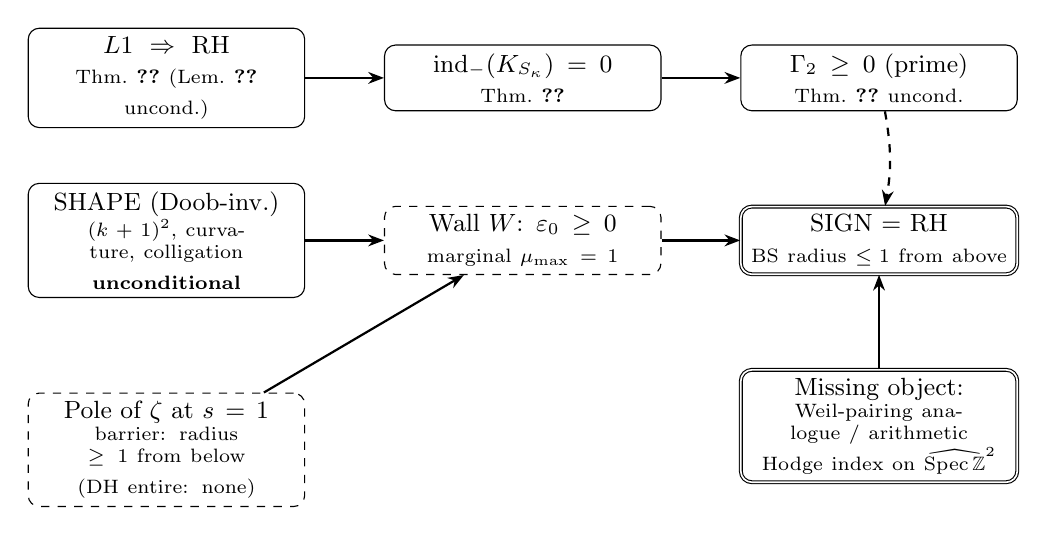
\begin{tikzpicture}[
   node distance=6mm and 10mm,
   box/.style={draw, rounded corners, align=center, font=\small, inner sep=3pt, text width=33mm},
   posb/.style={box},
   red/.style={box, dashed},
   open/.style={box, double},
   ar/.style={-{Stealth[length=2mm]}, thick}
]
\node[posb] (l1) {$L1\Rightarrow\RH$\\ \scriptsize Thm.~\ref{thm:L1} (Lem.~\ref{lem:pw} uncond.)};
\node[posb, right=of l1] (kl) {$\indm(K_{\Sk})=0$\\ \scriptsize Thm.~\ref{thm:kl}};
\node[posb, right=of kl] (cd) {$\Gamma_2\ge0$ (prime)\\ \scriptsize Thm.~\ref{thm:CD0} uncond.};
\node[red, below=12mm of kl] (wall) {Wall $W$: $\eps_0\ge0$\\ \scriptsize marginal $\mu_{\max}=1$};
\node[posb, left=of wall] (shape) {SHAPE (Doob-inv.)\\ \scriptsize $(k+1)^2$, curvature, colligation\\ \textbf{unconditional}};
\node[open, right=of wall] (sign) {SIGN $=$ RH\\ \scriptsize BS radius $\le1$ from above};
\node[open, below=12mm of sign] (weil) {Missing object:\\ \scriptsize Weil-pairing analogue / arithmetic\\ Hodge index on $\widehat{\Spec\Z}^2$};
\node[red, below=12mm of shape] (pole) {Pole of $\zeta$ at $s=1$\\ \scriptsize barrier: radius $\ge1$ from below\\ (DH entire: none)};

\draw[ar] (l1)--(kl); \draw[ar] (kl)--(cd);
\draw[ar] (shape)--(wall); \draw[ar] (pole)--(wall);
\draw[ar] (wall)--(sign); \draw[ar] (weil)--(sign);
\draw[ar, dashed] (cd) to[bend left=10] (sign);
\end{tikzpicture}
\end{center}
\noindent Solid boxes are unconditional; dashed boxes meet at the wall; double-ruled boxes are the
open content. The pole pins the Birman--Schwinger radius from below; the missing object would pin it
from above.

\subsection{What must be created}
The upper pinning is, in the function-field model, the \emph{Weil pairing}: Frobenius acts on
$H^1$ of a curve $C/\Fq$ as an isometry (up to $q$) of a positive intersection form, so its
eigenvalues lie on $|z|=\sqrt q$ (the curve RH). The $\Spec\Z$ analogue requires an arithmetic
intersection theory on the square of the Connes--Consani arithmetic site $\widehat{\Spec\Z}$ with
Frobenius correspondences $[F_t]$, a diagonal $[\Delta]$, and a Hodge-index sign, in which the
realization $f\mapsto Z_f$ satisfies $(Z_f\cdot Z_f)=W(f)$ (formally, by the trace formula) and
Abboud's arithmetic Hodge index $(D\cdot D)\le0$ for primitive $D$ applies. The degree condition
$(Z_f\cdot H)=0$ is exactly $\mu_{\max}=1$.

\medskip\noindent\textbf{Open target (the single remaining theorem, M3a).}
Construct $\widehat{\mathrm{CH}}^1(\widehat{\Spec\Z}^{\,2})$ with a symmetric pairing for which the
scaling correspondences $[F_t]$ and the diagonal are classes, $(Z_f\cdot Z_f)=W(f)$, and the
Hodge-index inequality holds; then RH. This is the Weil-pairing analogue over $\Spec\Z$; it does not
presently exist and must be \emph{created}.
\medskip

%% =====================================================================
\section{Synthesis}
%% =====================================================================
The route is assembled rigorously around a single arithmetic-geometric obstruction:
\[
   \RH\ \Longleftarrow\
   \underbrace{\big[\text{model space},\ \text{Lax--Phillips},\ \indm,\ \Gamma_2\ge0,\ \mu_{\max}=1,
   \ \text{Abboud}\big]}_{\text{rigorous / assembled}}\ \Longleftarrow\
   \underbrace{\text{M3a}}_{\text{open: the upper pinning}} .
\]
Three facts make this the honest endpoint. First, $L1\Rightarrow\RH$ (Theorem~\ref{thm:L1}):
the boundedness is not a lemma below RH, it is RH; the Laplace--pole obstruction is exactly the
off-line poles, so no analytic averaging can reach it (the Cesàro and monotone-continuation routes
are RH-equivalent). Second, $\Gamma_2\ge0$ (Theorem~\ref{thm:CD0}): the curvature/shape positivity
is unconditional and rooted in $\Lam\ge0$; the falsifier fails it. Third, the wall is the
\emph{sign} $\eps_0\ge0$, the Birman--Schwinger spectral radius pinned at $1$ --- from below by the
pole (which DH lacks), from above by the missing Weil-pairing analogue.

\begin{center}\itshape
The geometry proves the shape; RH is the sign; the sign is the upper pinning of the spectral radius;
the upper pinning is a piece of arithmetic geometry over $\Spec\Z$ that does not yet exist and must
be created.
\end{center}

%% =====================================================================
\section{Open problems}
%% =====================================================================
\begin{enumerate}[label=\textbf{O\arabic*.}]
\item \textbf{M3a (the upper pinning).} Construct the arithmetic intersection pairing on
$\widehat{\Spec\Z}^{\,2}$ with Frobenius correspondences and the Hodge-index sign. Candidate input:
the two-variable kernel $\xi(\half+iz)\xi(\half+iw)$ and the arithmetic-site Frobenius.
\item \textbf{Sharp curvature.} Is there a curvature-dimension refinement $CD(0,N)$ (finite $N$, from
the archimedean diffusion) that survives the Doob reduction and reaches $\eps_0$, or is the
Doob-invariance obstruction absolute?
\item \textbf{Positivity-improving with pinned radius.} Identify a structural reason the
pole-barriered von Mangoldt Birman--Schwinger kernel has spectral radius exactly $1$, analogous to
the Frobenius $\sqrt q$-isometry; this is the operator form of O1.
\item \textbf{Cyclicity for $L1$.} Prove the cyclicity/density of the near-radical windows needed for
the Jacobi-coordinate phrasing of Theorem~\ref{thm:L1} (the forward direction is already
coordinate-free).
\end{enumerate}

%% =====================================================================
\section{Conclusion}
%% =====================================================================
We carried the de~Branges/colligation route to its rigorous limit. The boundedness $L1$ is proved
equivalent to RH with an unconditional Paley--Wiener lemma; the correct invariant is the
Kre\u\i n--Langer index; the prime generator has unconditionally nonnegative Bakry--\'Emery
curvature by a Schur-product mechanism rooted in $\Lam\ge0$; and the wall is realized as a
pole-pinned Birman--Schwinger spectral radius, with the pole providing the lower pinning that the
Davenport--Heilbronn falsifier lacks. The remaining content is one object --- the Weil-pairing
analogue over $\Spec\Z$ --- which provides the upper pinning and which does not yet exist. Crossing
the wall is, precisely, creating it. Nothing here proves RH; the boundary is mapped exactly, and the
next step is an act of construction in arithmetic geometry.

%% =====================================================================
\begin{thebibliography}{99}
\bibitem{Connes} A.~Connes, \emph{Trace formula in noncommutative geometry and the zeros of the
Riemann zeta function}, Selecta Math. \textbf{5} (1999), 29--106.
\bibitem{CC} A.~Connes, C.~Consani, \emph{The Arithmetic Site}, C. R. Acad. Sci. Paris (2014); and
subsequent works on the scaling/arithmetic site.
\bibitem{CM} A.~Connes, H.~Moscovici, \emph{The UV prolate spectrum matches the zeros of zeta}
(2022).
\bibitem{deB} L.~de~Branges, \emph{Hilbert Spaces of Entire Functions}, Prentice-Hall, 1968.
\bibitem{SNF} B.~Sz.-Nagy, C.~Foia\c s, \emph{Harmonic Analysis of Operators on Hilbert Space},
North-Holland, 1970.
\bibitem{KL} M.~G.~Kre\u\i n, H.~Langer, \emph{\"Uber die verallgemeinerten Resolventen \dots},
Acta Sci. Math. (Szeged) (1977).
\bibitem{LP} P.~D.~Lax, R.~S.~Phillips, \emph{Scattering Theory}, Academic Press, 1967.
\bibitem{BE} D.~Bakry, M.~\'Emery, \emph{Diffusions hypercontractives}, S\'eminaire de
Probabilit\'es XIX (1985).
\bibitem{Weil} A.~Weil, \emph{Sur les ``formules explicites'' de la th\'eorie des nombres premiers},
Comm. S\'em. Math. Lund (1952).
\bibitem{Abboud} A.~Abboud, \emph{On the arithmetic Hodge index theorem} (arithmetic intersection
on arithmetic surfaces).
\end{thebibliography}

\end{document}
